\section{模块接口说明}
    \subsection{页式文件系统 DBFile}
        \begin{tabularx}{\textwidth}{lX}
            \toprule
            接口 & 描述 \\
            \midrule
            (constructor) & 接受文件名 \\
            \midrule
            create & 创建指定页大小的文件 \\
            \midrule
            remove & 删除文件 \\
            \midrule
            open & 打开文件 \\
            \midrule
            close & 关闭文件 \\
            \midrule
            writePage & 写指定页 \\
            \midrule
            readPage & 读指定页 \\
            \midrule
            isopen & 文件处于打开状态 \\
            \midrule
            accessible & 文件存在且有读写权限 \\
            \midrule
            pageSize & 返回页大小 \\
            \midrule
            numPages & 文件总页数 \\
            \bottomrule
        \end{tabularx}
    \subsection{缓冲区模块 DBBuffer}
        除在构造时接受缓冲区大小作为参数,其他与DBFile完全相同。

    \subsection{表属性管理 DBFields}
        \begin{tabularx}{\textwidth}{lX}
            \toprule
            接口 & 描述 \\
            \midrule
            insert & 添加一个属性 \\
            \midrule
            hasPrimaryKey & 有主键 \\
            \midrule
            addPrimaryKey & 添加隐藏主键 \\
            \midrule
            removePrimaryKey & 删除隐藏主键 \\
            \midrule
            size & 属性个数 \\
            \midrule
            recordLength & 记录总长度 \\
            \midrule
            field\_id & 所有属性ID \\
            \midrule
            field\_type & 所有属性类型 \\
            \midrule
            field\_length & 所有属性长度 \\
            \midrule
            field\_name & 所有属性名 \\
            \midrule
            indexed & 各属性是否有索引 \\
            \midrule
            notnull & 各属性取值是否不能为空 \\
            \midrule
            primary\_key\_field\_id & 主键ID \\
            \midrule
            datatypepe\_name\_map & 属性类型名称映射表 \\
            \midrule
            typeLength & 获取类型对应的默认长度 \\
            \midrule
            MinGenerator & 获取类型的最小可能取值 \\
            \midrule
            LiteralParser & 存储数据与显示数据之间转换 \\
            \midrule
            Comparator & 比较器 \\
            \bottomrule
        \end{tabularx}
    \subsection{系统管理 DBTableManager}
        \begin{tabularx}{\textwidth}{lX}
            \toprule
            接口 & 描述 \\
            \midrule
            create & 创建表 \\
            \midrule
            open & 打开表 \\
            \midrule
            isopen & 表处于打开状态 \\
            \midrule
            fildsDesc & 返回表属性描述 \\
            \midrule
            close & 关闭表 \\
            \midrule
            remove & 删除表 \\
            \midrule
            insertRecord & 插入一条记录 \\
            \midrule
            removeRecord & 删除一条记录 \\
            \midrule
            selectRecord & 查看一条记录 \\
            \midrule
            modifyRecord & 修改一条记录 \\
            \midrule
            traverseRecords & 遍历所有记录 \\
            \midrule
            findRecords & 查询满足条件的所有记录 \\
            \midrule 
            createIndex & 在某个属性创建索引 \\
            \midrule
            removeIndex & 删除某个属性的索引 \\
            \bottomrule
        \end{tabularx}
    \subsection{索引管理 DBIndexManager}
        \begin{tabularx}{\textwidth}{lX}
            \toprule
            接口 & 描述 \\
            \midrule
            (constructor) & 接受索引文件名 \\
            \midrule
            create & 创建索引 \\
            \midrule
            open & 打开索引 \\
            \midrule
            close & 关闭索引 \\
            \midrule
            remove & 删除索引 \\
            \midrule 
            searchRecord & 查找指定键值,返回该第一个该键值的RID \\
            \midrule
            searchRecords & 查找指定键值,返回所有该键值的RID \\
            \midrule
            rangeQuery & 范围查询 \\
            \midrule
            insertRecord & 插入一个键值 \\
            \midrule
            removeRecord & 删除第一个该键值 \\
            \midrule
            removeRecords & 删除所有该键值 \\
            \midrule
            traverseRecords & 遍历所有键值 \\
            \midrule
            getNumRecords & 返回键值总数 \\
            \bottomrule
        \end{tabularx}

    \subsection{命令执行 DBQuery}
        \begin{tabularx}{\textwidth}{lX}
            \toprule
            接口 & 描述 \\
            \midrule
            (constructor) & 接受标准输出和错误输出流 \\
            \midrule
            execute & 执行命令 \\
            \bottomrule
        \end{tabularx}

    \subsection{命令解析}
        较复杂,参见源文件。

    \subsection{错误处理 DBError}
        \begin{tabularx}{\textwidth}{lX}
            \toprule
            接口 & 描述 \\
            \midrule
            getInfo & 返回错误信息 \\
            \bottomrule
        \end{tabularx}

    \subsection{交互界面 DBInterface}
        \begin{tabularx}{\textwidth}{lX}
            \toprule
            接口 & 描述 \\
            \midrule
            feed & 输入数据到缓冲区中 \\
            \midrule
            ready & 指令已就绪 \\
            \midrule
            get & 取出一条指令 \\
            \midrule
            emptyBuff & 缓冲区为空 \\
            \bottomrule
        \end{tabularx}

    \begin{figure}[!hbp]
        \centering
        \caption{整体结构图}
        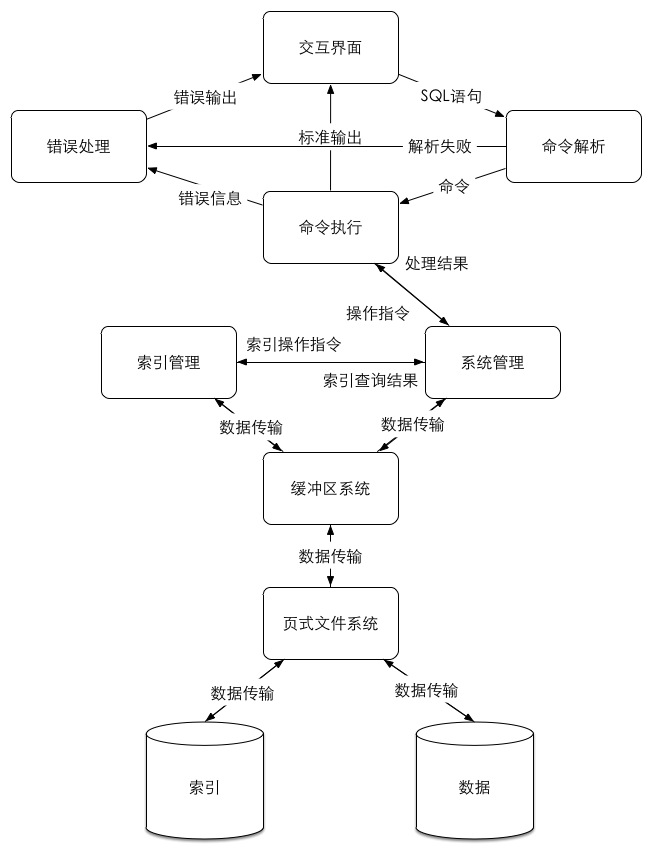
\includegraphics[width=0.9\textwidth]{chart/oursql.jpg}
    \end{figure}



